\documentclass[a4paper,12pt]{article}

%%% Работа с русским языком % для pdfLatex
\usepackage{cmap}					% поиск в~PDF
\usepackage{mathtext} 				% русские буквы в~фомулах
\usepackage[T2A]{fontenc}			% кодировка
\usepackage[utf8]{inputenc}			% кодировка исходного текста
\usepackage[english,russian]{babel}	% локализация и переносы
\usepackage{indentfirst} 			% отступ 1 абзаца
\usepackage{gensymb}				% мат символы?

%%% Работа с русским языком % для XeLatex
%\usepackage[english,russian]{babel}   %% загружает пакет многоязыковой вёрстки
%\usepackage{fontspec}      %% подготавливает загрузку шрифтов Open Type, True Type и др.
%\defaultfontfeatures{Ligatures={TeX},Renderer=Basic}  %% свойства шрифтов по умолчанию
%\setmainfont[Ligatures={TeX,Historic}]{Times New Roman} %% задаёт основной шрифт документа
%\setsansfont{Comic Sans MS}                    %% задаёт шрифт без засечек
%\setmonofont{Courier New}
%\usepackage{indentfirst}
%\frenchspacing

%%% Дополнительная работа с математикой
\usepackage{amsfonts,amssymb,amsthm,mathtools}
\usepackage{amsmath}
\usepackage{icomma} % "Умная" запятая: $0,2$ --- число, $0, 2$ --- перечисление
\usepackage{upgreek}

%% Номера формул
%\mathtoolsset{showonlyrefs=true} % Показывать номера только у тех формул, на которые есть \eqref{} в~тексте.

%%% Страница
\usepackage{extsizes} % Возможность сделать 14-й шрифт

%% Шрифты
\usepackage{euscript}	 % Шрифт Евклид
\usepackage{mathrsfs} % Красивый матшрифт

%% Свои команды
\DeclareMathOperator{\sgn}{\mathop{sgn}} % создание новой конанды \sgn (типо как \sin)
\DeclareMathOperator{\rg}{\mathop{rg}}
\DeclareMathOperator{\Rg}{\mathop{Rg}}
\DeclareMathOperator{\im}{\mathop{Im}}
\DeclareMathOperator{\tr}{\mathop{tr}}
\DeclareMathOperator{\const}{\mathop{const}}
\DeclareMathOperator{\Id}{\mathop{Id}}
%\DeclareMathOperator{\dim}{\mathop{dim}}
\usepackage{csquotes} % ещё одна штука для цитат
\newcommand{\pd}[2]{\ensuremath{\cfrac{\partial #1}{\partial #2}}} % частная производная
\newcommand{\abs}[1]{\ensuremath{\left|#1\right|}} % модуль
\renewcommand{\phi}{\ensuremath{\varphi}} % греческая фи
\newcommand{\pogk}[1]{\!\left(\cfrac{\sigma_{#1}}{#1}\right)^{\!\!\!2}\!} % для погрешностей


%\renewcommand{\labelenumi}{\asbuk{enumi})}

% Ссылки
\usepackage{color} % подключить пакет color
% выбрать цвета
\definecolor{BlueGreen}{RGB}{49,152,255}
\definecolor{Violet}{RGB}{120,80,120}
% назначить цвета при подключении hyperref
\usepackage[unicode, colorlinks, urlcolor=blue, linkcolor=blue, pagecolor=blue, citecolor=blue]{hyperref} %синие ссылки
%\usepackage[unicode, colorlinks, urlcolor=black, linkcolor=black, pagecolor=black, citecolor=black]{hyperref} % для печати (отключить верхний!)


%% Перенос знаков в~формулах (по Львовскому)
\newcommand*{\hm}[1]{#1\nobreak\discretionary{}
	{\hbox{$\mathsurround=0pt #1$}}{}}

%%% Работа с картинками
\usepackage{graphicx}  % Для вставки рисунков
\graphicspath{{images/}{images2/}}  % папки с картинками
\setlength\fboxsep{3pt} % Отступ рамки \fbox{} от рисунка
\setlength\fboxrule{1pt} % Толщина линий рамки \fbox{}
\usepackage{wrapfig} % Обтекание рисунков и таблиц текстом
\usepackage{multicol}

%%% Работа с таблицами
\usepackage{array,tabularx,tabulary,booktabs} % Дополнительная работа с таблицами
\usepackage{longtable}  % Длинные таблицы
\usepackage{multirow} % Слияние строк в~таблице
\usepackage{caption}
\captionsetup{labelsep=period, labelfont=bf}

%%% Оформление
\usepackage{indentfirst} % Красная строка
%\setlength{\parskip}{0.3cm} % отступы между абзацами
%%% Название разделов
\usepackage{titlesec}
\titlelabel{\thetitle.\quad}
\renewcommand{\figurename}{\textbf{Рис.}}		%Чтобы вместо figure под рисунками писал "рис"
\renewcommand{\tablename}{\textbf{Таблица}}		%Чтобы вместо table над таблицами писал Таблица
\usepackage{enumitem}
\setlist{nolistsep}
\usepackage{verbatim}

%%% Теоремы
\theoremstyle{plain} % Это стиль по умолчанию, его можно не переопределять.
\newtheorem{theorem}{Теорема}[section]
\newtheorem{proposition}[theorem]{Утверждение}
\newtheorem{predlog}{Предложение}[section]
\newtheorem{lemma}{Лемма}[section]

\theoremstyle{definition} % "Определение"
\newtheorem{definition}{Определение}[section]
\newtheorem{corollary}{Следствие}[theorem]
\newtheorem{problem}{Задача}[section]

\theoremstyle{remark} % "Примечание"
\newtheorem*{nonum}{Решение}
\newtheorem{zamech}{Замечание}[theorem]

%%% Правильные мат. символы для русского языка
\renewcommand{\epsilon}{\ensuremath{\varepsilon}}
\renewcommand{\phi}{\ensuremath{\varphi}}
\renewcommand{\kappa}{\ensuremath{\varkappa}}
\renewcommand{\le}{\ensuremath{\leqslant}}
\renewcommand{\leq}{\ensuremath{\leqslant}}
\renewcommand{\ge}{\ensuremath{\geqslant}}
\renewcommand{\geq}{\ensuremath{\geqslant}}
\renewcommand{\emptyset}{\varnothing}

%%% Для лекций по инфе
\usepackage{alltt}
\newcounter{infa}[section]
\newcounter{num}
\definecolor{infa}{rgb}{0, 0.2, 0.89}
\definecolor{infa1}{rgb}{0, 0.3, 1}
\definecolor{grey}{rgb}{0.5, 0.5, 0.5}
\newcommand{\tab}{\ \ \ }
\newcommand{\com}[1]{{\color{grey}\##1}}
\newcommand{\num}{\addtocounter{num}{1}\arabic{num}\tab}
\newcommand{\defi}{{\color{infa}def}}
\newcommand{\ini}{{\color{infa}in}}
\newcommand{\rangei}{{\color{infa}range}}
\newcommand{\fori}{{\color{infa}for}}
\newcommand{\ifi}{{\color{infa}if}}
\newcommand{\elsei}{{\color{infa}else}}
\newcommand{\printi}{{\color{infa1}print}}
\newcommand{\maxi}{{\color{infa}max}}
\newcommand{\classi}{{\color{infa}class}}
\newcommand{\returni}{{\color{infa}return}}
\newcommand{\elifi}{{\color{infa}elif}}


\newenvironment{infa}[1]{
	
	\vspace{0.5cm}
	\addtocounter{infa}{1}%
	\noindent{\large \textbf{Программа №\thesection.\arabic{infa}}}\textbf{<<#1>>}%
	\begin{alltt}%
	}{\end{alltt}
	\setcounter{num}{0}
	\vspace{0.1cm}}
%Пример кода:
%\begin{infa}{Поразрядная сортировка}
%	\ \num \defi count_sort(a):\tab \com{определяет нашу функцию}
%	\ \num \tab m = \maxi(a)+1
%	\ \num \tab q = [0]*m
%	\ \num \tab \fori x \ini a:
%	\ \num \tab \tab q[x] += 1
%	\ \num \tab pos = 0
%	\ \num \tab \fori x \ini q:
%	\ \num \tab \tab \fori i \ini \rangei(q[x]):
%	\ \num \tab \tab \tab a[pos] = x
%	\num \tab \tab \tab pos += 1
%\end{infa}

\usepackage{titlesec}
\titlelabel{\thetitle.\quad}


\usepackage{graphicx,xcolor,adjustbox,setspace}

\newcommand{\resh}{\noindent\textit{Решение:}\\}

\newcounter{prim}
\newenvironment{prim}{%
	\addtocounter{prim}{1}
	\noindent{\\
		\textbf{\noindentПример \arabic{prim}\\}}%
}{\vspace{2mm}\\
\resh
}
\definecolor{orange}{rgb}{1, 0.7, 0.1}
%\usepackage{ulem}

\usepackage{bm} %жирный греческий шрифт

\newenvironment{psm}
{\left(\begin{smallmatrix*}[r]}
	{\end{smallmatrix*}\right)}

\newenvironment{pmatrixr}
{\begin{pmatrix*}[r]}
	{\end{pmatrix*}}

\renewcommand{\figurename}{\textbf{Рис.}}		%Чтобы вместо figure под рисунками писал "рис"
\renewcommand{\tablename}{\textbf{Таблица}}		%Чтобы вместо table над таблицами писал Таблица


\title{Lab 2.3.1}
\author{Кожарин Алексей}
\date{May 2017}
\usepackage[left=1.27cm,right=1.27cm,top=1.27cm,bottom=2cm]{geometry}

\begin{document}

\begin{titlepage}
	\begin{center} 
		
		\large Московский физико-технический институт\\
		Факультет молекулярной и химической физики\\
		\vspace{7cm}
		\huge Лабораторная работа №2.3.1\\
		\textbf{\Large <<Получение и измерение вакуума>>}\\
	\end{center} 
	
	\vspace{7.5cm}
	{\par \raggedleft \large \emph{Выполнил:}\\ студент 1 курса\\ 642 группы ФМХФ\\ Кожарин Алексей\\ Сергеевич  \par}
	\begin{center}
		\vfill Москва 2017
	\end{center}
\end{titlepage}
\newpage
\setcounter{page}{2}

\begin{center}
	\vspace*{-0.5cm}{
		\textbf{Аннотация:}\\ 
		\vspace{0.2cm}
		\parbox{16cm}{ 
			\tab В~этом отчёте изложены результаты выполнения лабораторной работы <<Получение и измерение вакуума>>. С помощью установки, состоящей из форвакуумной и высоковакуумной частей мы получаем высокий вакуум ($p \sim  10^{-4} $ торр), а затем измеряем параметры установки: объемы всех ее частей и скорость откачки в стационарном режиме, при ухудшении и улучшении вакуума. Для этого мы создаем искусственную течь.
		}
	}
\end{center}
\hspace{0.2cm}\textbf{Цель работы:}
\par 1) измерение объёмов форвакуумной и высоковакуумной частей установки;
\par 2) определение скорости откачки системы в стационарном режиме, а также при ухудшении и 
улучшении вакуума.

\textbf{\section{1. Теоретическое введение}}
По степени разрежения вакуумные установки принято делить на три класса: 1) низковакуумные -- до $10^{-2}-10^{-3}$ торр; 2) высоковакуумные -- $10^{-4} - 10^{-7}$ торр; 3) установки сверхвысокого вакуума -- $10^{-8} - 10^{-11}$ торр. С физической точки зрения низкий вакуум переходит в высокий, когда длина свободного пробега молекул газа оказывается сравнима с размерами установки (а течение газа становится сугубо молекулярным); сверхвысокий вакуум характерен крайней важностью процессов адсорбции и десорбции частиц на поверхности вакуумной камеры.
\par В данной работе изучаются традиционные методы откачки механическим форвакуумным насосом до давления $10^{-2}$ торр и диффузионным масляным насосом до давления $10^{-5}$ торр, а также~методы~измерения~вакуума~в этом диапазоне.

\textbf{\section{2. Экспериментальная установка}}
\begin{figure}[h]
	\center{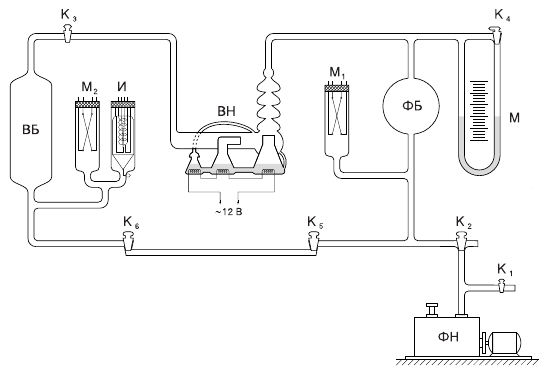
\includegraphics[width=0.8\linewidth]{scheme}}
	\caption{Схема экспериментальной установки}
	\label{r1}
\end{figure}                      
Установка изготовлена из стекла
и состоит из форвакуумного баллона (ФБ), высоковакуумного диффузионного насоса (ВН), высоковакуумного баллона (ВБ), масляного (М) и ионизационного (И) манометров, термопарных манометров
(М1 и M2), форвакуумного насоса (ФН) и соединительных кранов К1 ,
К2 , ... , К6 (см. рис. \ref{r1}).
\par \emph{Краны}. Все краны вакуумной установки — стеклянные. Стенки
кранов тонкие, пробки кранов — полые и составляют одно целое с рукоятками. Для герметизации используется вакуумная смазка. 
\par Кран К1 используется для заполнения форвакуумного насоса и вакуумной установки атмосферным воздухом. Трехходовой кран К2 служит для соединения форвакуумного насоса с установкой или атмосферой. Кран К3 отделяет высоковакуумную часть установки от форвакуумной.
Кран К4 соединяет между собой колена масляного манометра Краны К5 и
К6 стоят по концам капилляра и соединяют его с форвакуумной и
высоковакуумной частями установки.
\par \emph{Форвакуумный насос}. Устройство, обеспечивающее механическую откачку воздуха до $10^{-2}$ торр, называется форвакуумным насосом. Его использование необходимо для того, чтобы подготовить подходящие условия для работы диффузионного насоса. Схематически принцип работы форвакуумного насоса изображен на рис. \ref{r2}.\\
\begin{figure}[h]
	\center{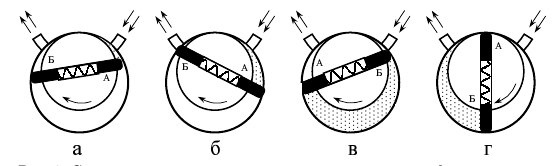
\includegraphics[width=0.9\linewidth]{nasos}}
	\caption{
		Схема форвакуумного насоса. В положениях <<a>> и <<б>> пластина <<A>> засасывает разреженный воздух из откачиваемого объёма, а пластина <<Б>> вытесняет ранее захваченный воздух в атмосферу. В положениях <<в>> и <<г>> пластины поменялись ролями
	}
	\label{r2}
\end{figure} 
\begin{wrapfigure}{r}{0.39\textwidth}
		\fbox{
			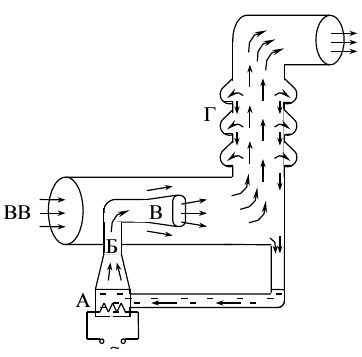
\includegraphics[width=\linewidth]{nasos1}}
		\caption{Схема работы диффузионного насоса}
		\label{r3}
	\vspace{-1.4cm}
\end{wrapfigure}
\par \emph{Диффузионный насоc}. Откачивающее действие диффузионного насоса основано на диффузии молекул разреженного воздуха в струю паров масла. Попавшие в струю молекулы газа увлекаются ею и уже не возвращаются назад. Это и создает откачивающее действие. Схематически это изображено на рис. \ref{r3}. Диффузионный насос, используемый в нашей установке, имеет две ступени и соответственно два сопла. Одно сопло
вертикальное (первая ступень), второе сопло горизонтальное (вторая
ступень).
\textbf{\section{3. Процесс откачки}}
\par Рассмотрим обычную схему откачки. Обозначим через $Q_\text{д}$ количество газа, десорбирующегося с поверхности откачиваемого объема в
единицу времени, через $Q_\text{и}$ — количество газа, проникающего в единицу времени в этот объем извне — через течи. Будем считать, что
насос обладает скоростью откачки W и в то же время сам является источником газа; пусть $Q_\text{н}$ — поток газа, поступающего из насоса
назад в откачиваемую систему. Будем измерять количество газа $Q_\text{д}$,
$Q_\text{н}$ и $Q_\text{и}$ в единицах $PV$ (легко видеть, что это произведение с точностью до множителя $RT /\mu$ равно массе газа). Основное уравнение, описывающее процесс откачки, имеет вид:
\begin{equation}
-VdP = (PW - Q_\text{д} - Q_\text{н} - Q_\text{и})dt
\label{eq1}
\end{equation}
При достижении предельного вакуума:
\begin{equation}
\cfrac{dP}{dt} = 0
\nonumber
\end{equation}
так что
\begin{equation}
P_\text{пр}W = Q_\text{д} + Q_\text{н} + Q_\text{и}
\label{eq2}
\end{equation}
Отсюда скорость откачки через предельный вакуум:
\begin{equation}
W = \cfrac{\sum Q_i}{P_\text{пр}}
\nonumber
\end{equation}
Считая $Q_\text{и}$, $Q_\text{н}$, $Q_\text{д}$ постоянным, уравнение (\ref{eq1}) можно проинтегрировать и, используя (\ref{eq2}), получить
\begin{equation}
P - P_\text{пр} = (P_0 - P_\text{пр})~\text{exp}\left(-\cfrac{W}{V}\,t\right)
\end{equation}
где $P_0$ --- начальное давление. Оно велико по сравнению с $P_\text{пр}$, поэтому имеем:
\begin{equation}
P = P_0~\text{exp}\left(-\cfrac{W}{V}\,t\right)
\label{eq_p}
\end{equation}
Постоянная времени откачки $\tau = \cfrac{V}{W}$ является мерой эффективности откачной системы. \\
Для количества газа, протекающего через трубу в условиях высокого вакуума, справедлива формула:
\begin{equation}
\cfrac{d(PV)}{dt} = \cfrac{4}{3}\,r^3 \sqrt{\cfrac{2\pi RT}{\mu}} \cfrac{P_2-P_1}{L}
\label{dPV}
\end{equation}
Теория и рисунки взяты из \cite{Gladun:PrakMech}
\textbf{\section{4. Обработка данных}}
\begin{spacing}{1.4}
По перепаду давлений в U-образном манометре находим объём форвакуумной и высоковакуумной части по формуле $P_0 V_0 = P_1 V_1$,\\ где $P_1 = \rho_M g \Delta h$,~~ $\rho_M = 0.886 \cfrac{\text{г}}{\text{см}^3}$,~~ $g=9.8 \cfrac{\text{м}}{\text{c}^2}$ \\
$\Delta h_\text{фв} = 14.5~\text{см} \rightarrow$ \fbox{$V_\text{фв} = 3040 ~\text{см}^3$} \\
$\Delta h_\text{вв+фв} = 10.75~\text{см} \rightarrow V_\text{вв+фв} = 4100 ~\text{см}^3 \Rightarrow$ \fbox{$V_\text{вв} = 1060 ~\text{см}^3$}
\end{spacing}
Минимальное давление, которое можно получить только лишь с использованием форвакуумного насоса, равно $p_\text{min} = 1.6 \cdot 10^{-2}$ торр. Для него длина свободного пробега \vspace*{0.2cm} \\
$\lambda_1 = \cfrac{1}{n\sigma} = \cfrac{kT}{P\pi d^2} = 4.7$ см 
\par Для высоковакуумной установки можно получить давление $p_\text{min} = 2.2 \cdot 10^{-4}$ торр. Для него \\
$\lambda_2 = 1.2$ м
\par Для эксперимента с улучшением вакуума, как следует из формулы (\ref{eq_p}), строим график $\ln(p/p_0) (t)$:

\begin{table}%FIXME поправить таблицы
	\centering
\begin{tabular}{|c|c|c|c|}
	\hline
	$t$, с & $\mu A$, мА & $p \cdot 10^{-4}$, торр & $\ln(p/p_0)$ \\ \cline{1-4}
	0 & 91 &  9,1 & 0 \\\cline{1-4}
	2 & 78 &  7,8 & -0,1541 \\\cline{1-4}
	4 & 67 &  6,7 & -0,3061 \\\cline{1-4}
	6 & 59 &  5,9 & -0,4333 \\ \cline{1-4}
	8 & 52 &  5,2 & -0,5596 \\\cline{1-4}
	10 & 48 &  4,8 & -0,6396 \\\cline{1-4}
	12 & 44 &  4,4 & -0,7266 \\\cline{1-4}
	14 & 40 &  4,0 & -0,8219 \\\cline{1-4}
	16 & 38 &  3,8 & -0,8732 \\\cline{1-4}
	18 & 35 &  3,5 & -0,9555 \\\cline{1-4}
	20 & 33 &  3,3 & -1,0143 \\ \cline{1-4}
	22 & 32 &  3,2 & -1,0451 \\\cline{1-4}
	24 & 30 &  3,0 & -1,1096 \\\cline{1-4}
	26 & 29 &  2,9 & -1,1435 \\\cline{1-4}
	28 & 28,5 &  2,9 & -1,1609 \\\cline{1-4}
	30 & 28 &  2,8 & -1,1786 \\\cline{1-4}
	32 & 27 &  2,7 & -1,2150 \\\cline{1-4}
	34 & 26 &  2,6 & -1,2527 \\\cline{1-4}
	36 & 26 &  2,6 & -1,2527 \\\cline{1-4}
	38 & 25,5 &  2,6 & -1,2721 \\\cline{1-4}
	40 & 25 &  2,5 & -1,2919 \\\cline{1-4}
	42 & 25 &  2,5 &-1,2919 \\ \cline{1-4}
\end{tabular}
	\caption{Значения, полученные при проведении эксперимента}
	\label{Tab:tab_exp}
\end{table}

\begin{figure}[h]
	\center{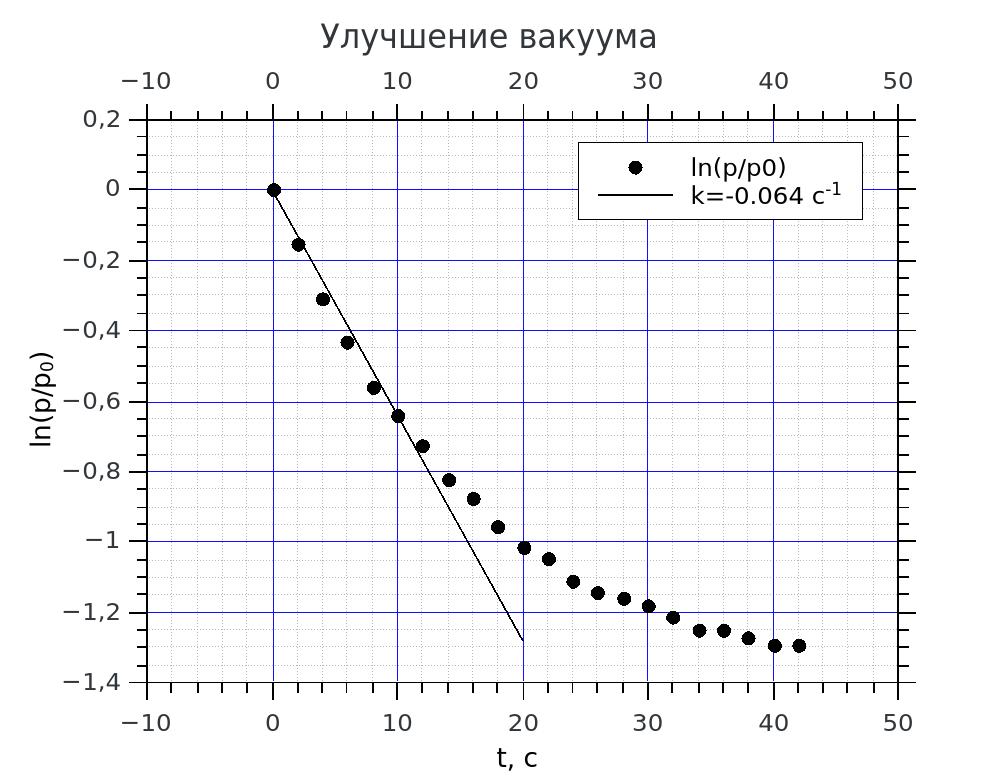
\includegraphics[width=0.9\linewidth]{graph_b}}
	\caption{
		Эксперимент с улучшением вакуума.
	}
	\label{g1}
\end{figure}
\newpage
Видно, что для больших промежутков времени теоретическая зависимость нарушается. Вероятнее всего, это связано с неприменимостью формулы (\ref{eq_p}) для почти стационарного процесса. Поэтому имеет смысл проводить аппроксимацию по первым точкам. По наклону определяем скорость откачки системы: \vspace{0cm}
\begin{center}
	\fbox{$W = -V \cdot k = 67.8 ~\cfrac{\ \text{см}^3}{\text{c}}$}
\end{center} \vspace{0.2cm}
\par Зная $p_\text{min}$ и $W$, можно определить по (\ref{eq2}) $Q_\text{д} + Q_\text{н} + Q_\text{и}$:
\begin{center}
 \fbox{
$Q_\text{д} + Q_\text{н} + Q_\text{и} = 1.49 \cdot 10^{-2} ~\cfrac{\text{торр}\cdot \text{см}^3}{\text{с}}$}
\end{center}
\par По эксперименту с ухудшением вакуума можно судить о $Q_\text{д} + Q_\text{и}$:
\begin{table}%FIXME поправить таблицы
	%\vspace{-0.5cm}
	\centering
\begin{tabular}{|c|c|c|c|}
	\hline
	$t$, с & $\mu A$, мА & $p$, торр $\cdot 10^{-4}$ \\ \cline{1-3}
	0 & 22 & 2,2 \\ \cline{1-3}
	2 & 26 &  2,6 \\ \cline{1-3}
	4 & 29 &  2,9 \\ \cline{1-3}
	6 & 32 &  3,2 \\ \cline{1-3}
	8 & 34,5 &  3,45 \\ \cline{1-3}
	10 & 38 &  3,8 \\ \cline{1-3}
	12 & 40,5 &  4,05 \\ \cline{1-3}
	14 & 43 &  4,3 \\ \cline{1-3}
	16 & 46 &  4,6 \\ \cline{1-3}
	18 & 49 &  4,9 \\ \cline{1-3}
	20 & 51,5 &  5,15 \\ \cline{1-3}
	22 & 54 &  5,4 \\ \cline{1-3}
	24 & 57 &  5,7 \\ \cline{1-3}
	26 & 59,5 &  5,95 \\ \cline{1-3}
	28 & 62,5 &  6,25 \\ \cline{1-3}
	30 & 65 &  6,5 \\ \cline{1-3}
	32 & 68 &  6,8 \\ \cline{1-3}
	34 & 71 &  7,1 \\ \cline{1-3}
	36 & 73 &  7,3 \\ \cline{1-3}
	38 & 76,5 & 7,65 \\ \cline{1-3}
	40 & 78,6 &  7,86 \\ \cline{1-3}
	42 & 82 &  8,2 \\ \cline{1-3}
	44 & 84 &  8,4 \\ \cline{1-3}
	46 & 86 &  8,6 \\ \cline{1-3}
	48 & 89 &  8,9 \\ \cline{1-3}
\end{tabular}
	\caption{Табличные данные и значения, полученные при проведении эксперимента}
	\label{Tab:tab_exp}
\end{table}
\vspace{-1cm}
\begin{figure}[h!]
	\center{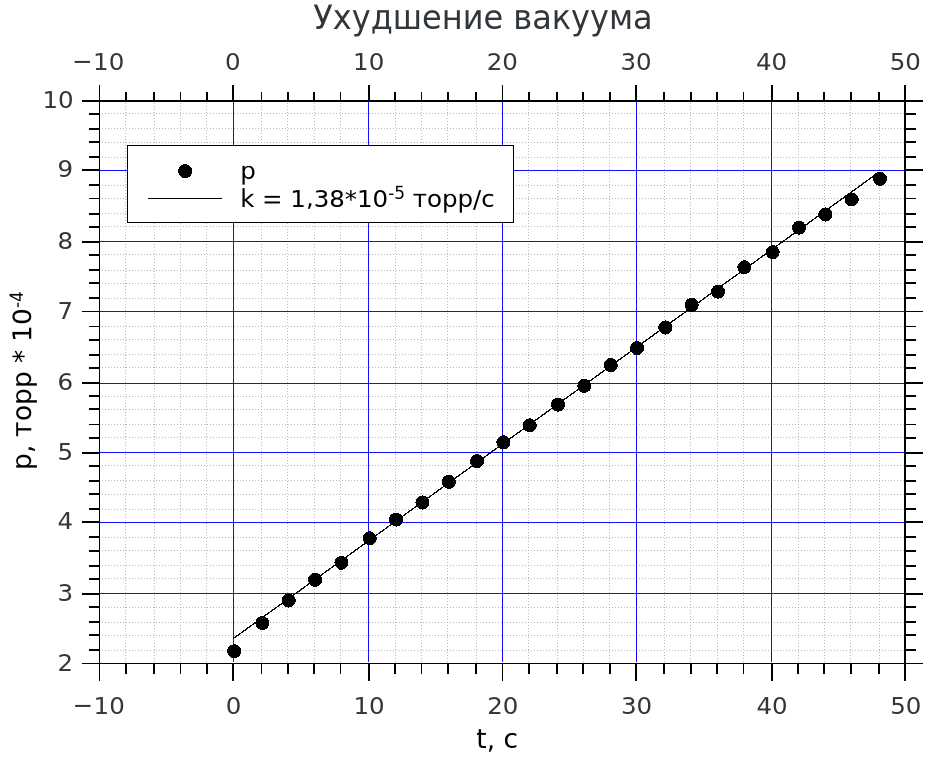
\includegraphics[width=0.9\linewidth]{graph_w}}
	\caption{
		Эксперимент с ухудшением вакуума.
	}
	\label{g2}
\end{figure}
\newpage
Пользуясь формулой $V_\text{вв} \cfrac{dP}{dt} = Q_\text{д} + Q_\text{и}$, находим \fbox{$ Q_\text{д} + Q_\text{и} = 1.46 \cdot 10^{-2} ~\frac{\text{торр}\cdot\text{см}^3}{\text{с}}$} \\
Отсюда сразу \fbox{$Q_\text{н} = 3 \cdot 10^{-4}~\frac{\text{торр}\cdot\text{см}^3}{\text{с}}$}
\par По полученным данным можно посчитать пропускную способность трубы:
\begin{equation}
C_\text{тр} = \left(\cfrac{dV}{dt}\right)_\text{тр} = \cfrac{4}{3} \cfrac{r^3}{L} \sqrt{\cfrac{2\pi RT}{\mu}} = 2.18 \cdot 10^{-1} ~\cfrac{\ \text{м}^3}{\text{с}}
\label{eq_C}
\end{equation}
\par Видно, что $W \ll C_\text{тр}$ --- газ сильно разрежен.
\par Для эксперимента с искусственной течью через капилляр воспользуемся формулой (\ref{dPV}):
\begin{center}
\hspace*{0.7cm}\fbox{$\frac{d(PV)}{dt} = 1.29 \cdot 10^{-2}~\frac{\text{торр}\cdot\text{см}^3}{\text{с}}$}
\end{center}
\par Попробуем пойти несколько в обратном направлении. Зная $P_\text{пр}$, $P_\text{уст}$ и $\frac{d(PV)}{dt}$, можно составить систему:
$$\left\{
\begin{array}{l}
P_\text{пр} W = Q_1\\
P_\text{уст} W = Q_1 + \cfrac{d(PV)_\text{капп}}{dt}\\
\end{array}
\right.$$
Разрешая её относительно $W$ и $Q_1 = Q_\text{д} + Q_\text{н} + Q_\text{и}$, получаем:
\begin{center}
$W = 61.4 ~\frac{\text{см}^3}{\text{с}}$ \\
$Q_1 = 1.35 \cdot 10^{-2} ~\frac{\text{торр}\cdot \text{см}^3}{\text{с}} $ \\
\small{\emph{(Здесь мы учли, что, $p_u = 4.3 \cdot 10^{-4}~ \text{торр}$)}} \end{center}
\vspace{100cm}
\textbf{\section{5. Заключение}}
В данной работе рассматривалось получение вакуума в две стадии. 

После измерения параметров установки были получены следующие значения: 
 \\
\begin{center}
\par \fbox{\parbox{\dimexpr\linewidth-136\fboxsep-2\fboxrule\relax}{ $p_\text{пред} = 2.2 \cdot 10^{-4} ~\text{торр} \\
		W = 67.8 ~\frac{\ \text{см}^3}{\text{c}}$ \\
		$Q = 1.49 \cdot 10^{-2} ~\frac{\text{торр}\cdot \text{см}^3}{\text{с}} $
	}}.
\end{center}
\bibliography{mybibliography}	
\bibliographystyle{gost705}

\end{document}
